\section{Case Study: Real-time feedback control of a hex-rotor with contract based estimation and robust control}
\label{experiments}

To evaluate our methodology on a real platform, we applied it to a hex-rotor tasked with following a given trajecotory. The hex-rotor flies using visual odometry from a downward facting camera for self-localization and using our Robust Model Predictive Algorithm for both the position control of the hex-rotor and setting the time deadline for the visual odometry computations. For the contract based perception and estimation algorithm we use the FAST corner detector (as in section \ref{}) providing measurements to an Unscented Kalman Filter that also uses measurements from an Inertial Measurement Unit (IMU) to provide a state estimate for the control algorithm to use.
In the following section we show how our approach dynamically schedules different modes of the contract-based perception and estimation algorithm at run-time and also controls the dynamic system in an energy efficient order while providing good tracking performance. In the evaluation subsection we will compare our results to a baseline Model Predictive Control algorithm that does not leverage co-design and operates at fixed ($\delta,\epsilon$) points of the perception/estimation algorithm which provides a state estimate to the controller. 

\subsection{Experimental setup}
\todo[inline]{details about hex-rotor and odroid and the visual odometry. Figure for control/percpetion architecture of hex-rotor here}
%Hexrotor \textbf{<specs here>} using visual odometry from a downward facing camera. Figure for hexrotor, figure for images from hexrotor downward facing, and figure for hexrotor control architecture.  

%We illustrate the foregoing results on the hexarotor example from Section \ref{motivatingExample}.
%Recall that we found the control performance, as measured by $J$ of Eq.??, to degrade as the robot's speed was increased.
%We implemented the RAMPC controller of Section \ref{controlProblem}, and used the error-delay curves of Section \ref{delayErrorCurve}.


\subsection{Profiing the perception and algorithm toolchain}

\begin{figure}[htbp]
  \centering
  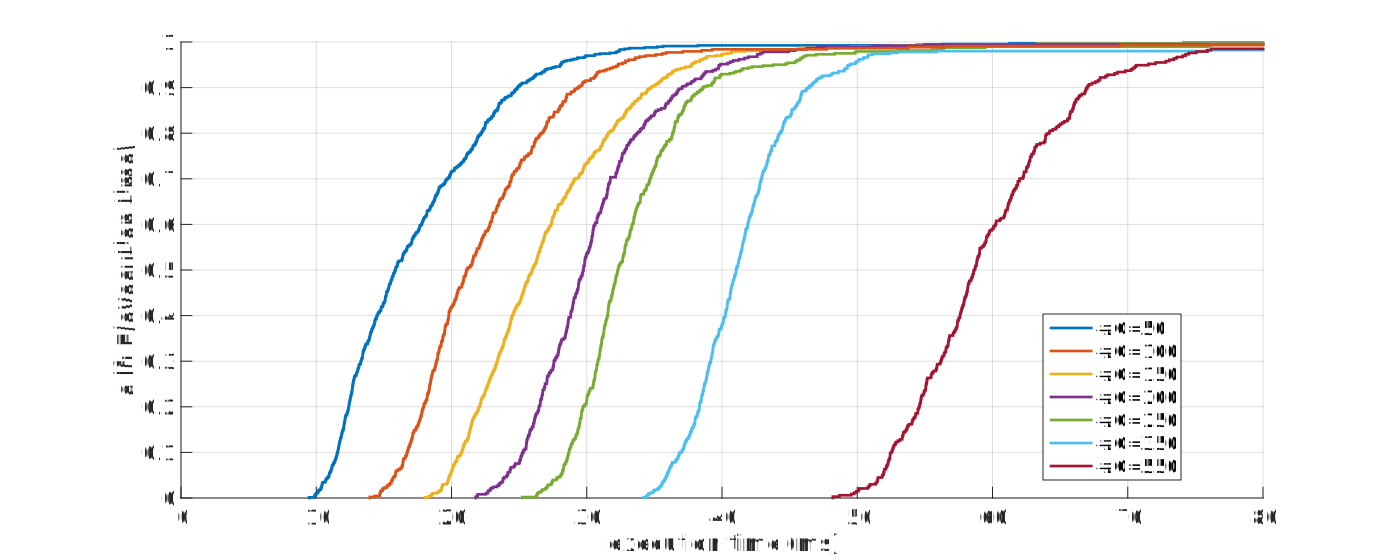
\includegraphics[width=0.45\textwidth]{figures/time_ecdf_millisec.pdf}
  \caption{Cumulative distribution of profiled execution times for visual odometry running on the Odroid U-3 for varying maximum number of corners from the FAST detector.}
\end{figure}

For the same sequence of increasing speeds (which translates to more stringent control demands), RAMPC performs better than MPC as illustrated in Fig.\ref{fig:RAMPCcost}.
\begin{figure}[t]
	\centering
	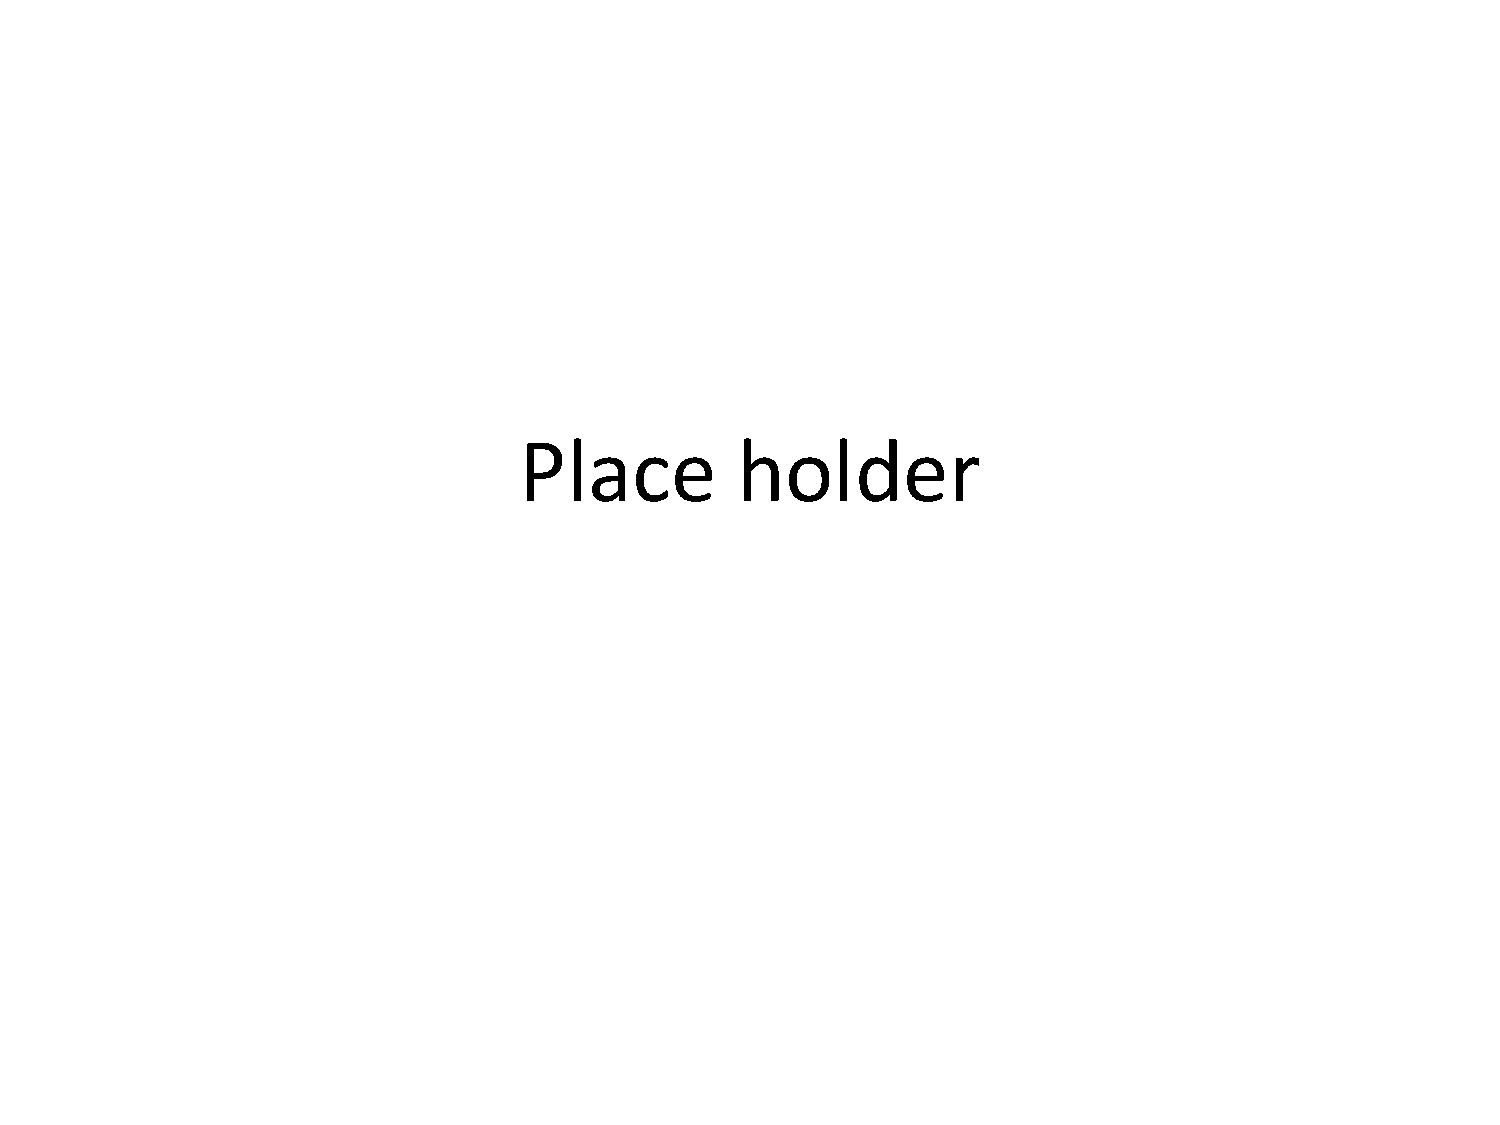
\includegraphics[width=0.7\linewidth]{figures/placeHolder}
	\caption{Cost function of RAMPC.}
	\label{fig:RAMPCcost}
\end{figure}

Fig.~\ref{fig:RAMPCtrajectory} shows the reference and actual trajectories of the hexarotor under RAMPC control.
\begin{figure}[t]
	\centering
	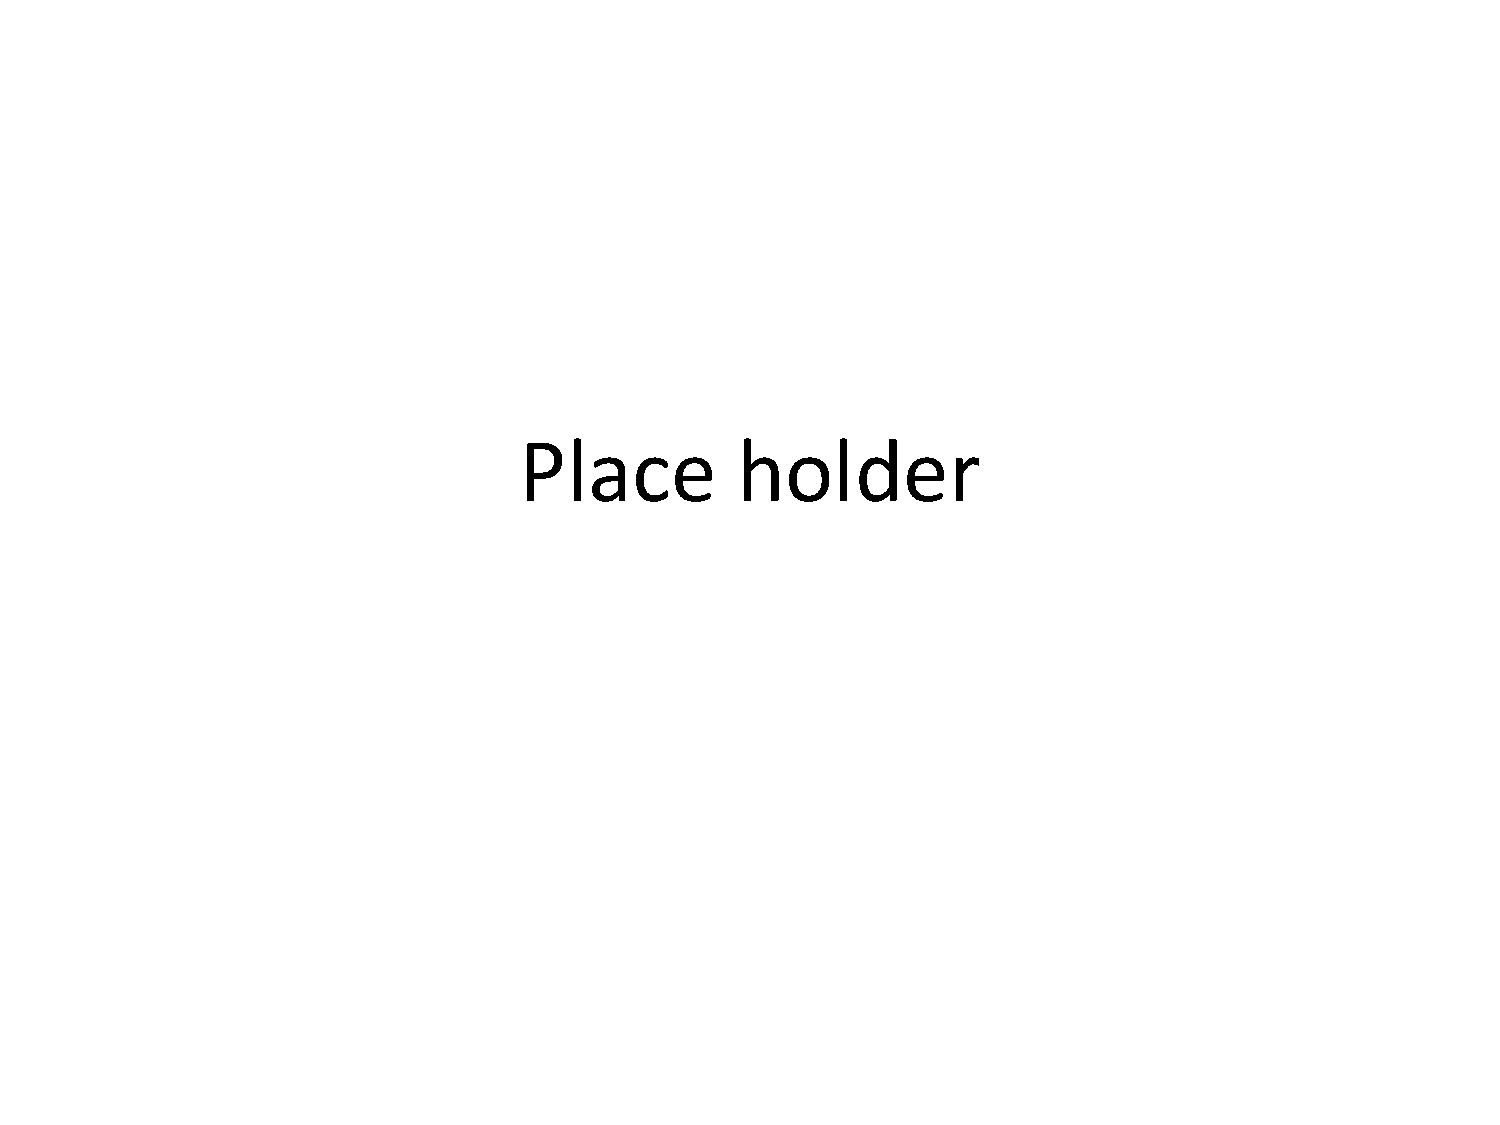
\includegraphics[width=0.7\linewidth]{figures/placeHolder}
	\caption{Reference and actual hexarotor trajectories controlled by RAMPC.}
	\label{fig:RAMPCtrajectory}
\end{figure}

Fig.~\ref{fig:modeSwitching} shows that the RAMPC indeed chooses different modes, indicating that awareness of the error/delay trade-off does lead to improved performance.
\begin{figure}[t]
	\centering
	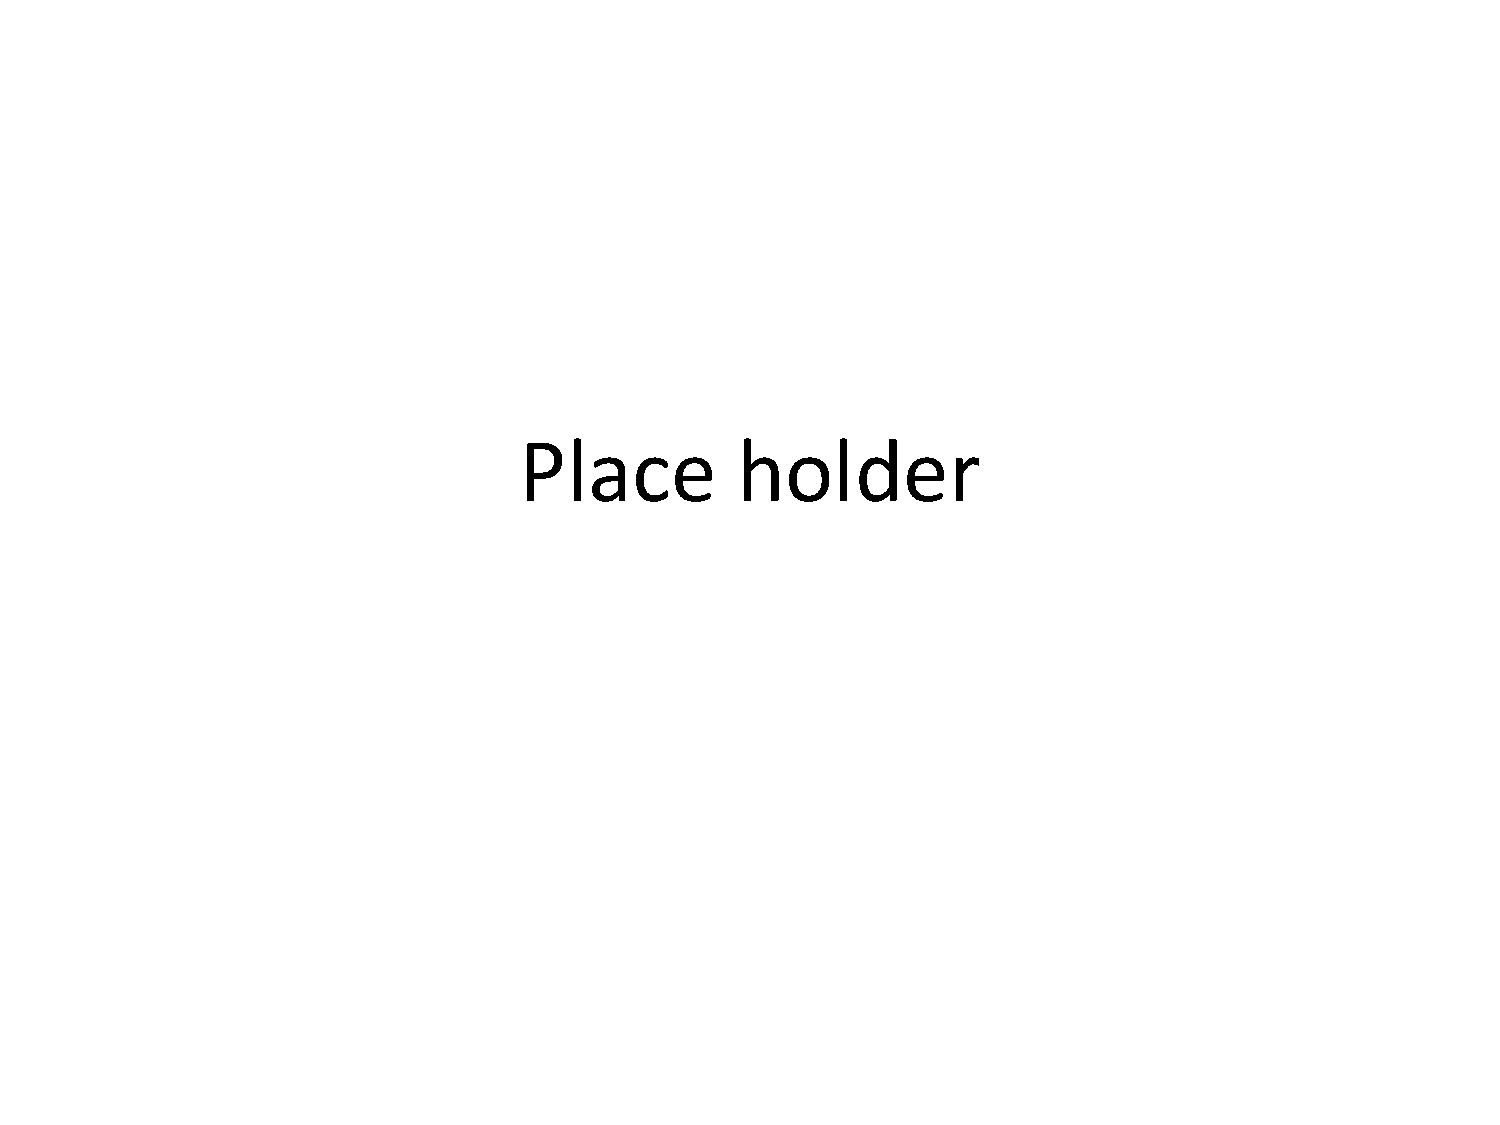
\includegraphics[width=0.7\linewidth]{figures/placeHolder}
	\caption{Mode switches of RAMPC.}
	\label{fig:modeSwitching}
\end{figure}
